{SoftIron}

\hypertarget{usb-console}{%
\section{USB Console}\label{usb-console}}

As HyperDrive nodes are specially designed to operate in a datacenter,
they do not have the video, keyboard, or mouse connections typically
found on PCs. The most simple way to interact with a HyperDrive node is
by connecting to the on-board USB B connector located on the back of the
case. Using a software terminal emulator, this connector will give the
user a connection to the main console of the node. All boot and UEFI
messages and menus will be seen on this console, and a login prompt will
be presented after boot. Additionally, in the event a node becomes
inaccessible from the network (due to setting a bad IP address, for
example), the USB console can always be used to regain access.

This console connection could, for example, be connected temporarily to
a debug laptop as and when necessary, or it could be connected
permanently to a terminal server to be used for routine maintenance.

The use of the USB console is optional for normal operation. If the
network is configured properly, IPMI or SSH could instead be used for
all maintenance functions

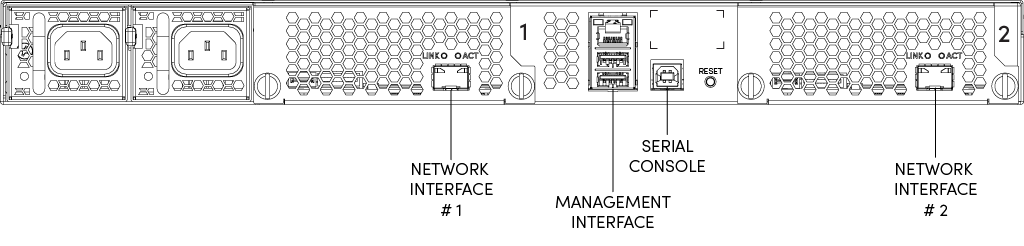
\includegraphics{/assets/bitmaps/2156e963-1c41-4780-b97d-b83a2e07294e.png}

\hypertarget{console-connection}{%
\subsection{\texorpdfstring{\protect\hyperlink{console-connection}{\#}
Console Connection}{\# Console Connection}}\label{console-connection}}

Using this console from a host PC is different on each host operating
system. Since the console uses USB, settings like baud rate, data bits,
and stop bits do not need to be specified.

To catch all the boot messages, it's advisable to start up a terminal
program on the host PC and connect it to the HyperDrive's USB console
before powering the HyperDrive on.

\hypertarget{linux}{%
\subsubsection{\texorpdfstring{\protect\hyperlink{linux}{\#}
Linux}{\# Linux}}\label{linux}}

On Linux systems, no special drivers are required. A number of terminal
emulator programs support serial consoles including \texttt{picocom} and
\texttt{screen}. The device path to the serial console of the most
recently connected node must first be identified. dmesg -w will display
kernel messages live, and USB devices will appear here as they are
plugged in. Alternatively, to view a list of all currently connected and
mapped serial consoles, run:

\begin{verbatim}
# ls -al /dev/serial/by-id/
\end{verbatim}

If there are SoftIron servers connected by serial, the output will look
something like:

\begin{verbatim}
lrwxrwxrwx 1 root root  13 Jun 17 18:04 usb-SoftIron_BMC_e0fff7001342-if00 -> ../../ttyACM2
lrwxrwxrwx 1 root root  13 Jun 17 18:04 usb-SoftIron_BMC_e0fff70013db-if00 -> ../../ttyACM0
lrwxrwxrwx 1 root root  13 Jun 17 18:04 usb-SoftIron_BMC_e0fff7001433-if00 -> ../../ttyACM5
\end{verbatim}

So that they're easy to identify, the nodes are mapped with their
on-board BMC MAC address in the name. The node with the BMC MAC of
\texttt{E0:FF:F7:00:13:42} can now be connected to over
\texttt{/dev/ttyACM2}.

Picocom can now be used as root to connect over serial to the node:

\begin{verbatim}
# picocom /dev/ttyACM2/
\end{verbatim}

\hypertarget{macos}{%
\subsubsection{\texorpdfstring{\protect\hyperlink{macos}{\#}
MacOS}{\# MacOS}}\label{macos}}

For MacOS, the device path can be identified with:

\begin{verbatim}
ls /dev/tty* | grep serial
\end{verbatim}

Screen can then be used:

\begin{verbatim}
screen /dev/tty.usbserial-A6004byf
\end{verbatim}

\hypertarget{windows}{%
\subsubsection{\texorpdfstring{\protect\hyperlink{windows}{\#}
Windows}{\# Windows}}\label{windows}}

To connect to the serial console from Windows, Device Manager can be
used to identify the correct COM port. If correctly connected, the
device should appear underneath "Ports (COM \& LPT)", and be labeled
with the correct COM number

\href{https://www.chiark.greenend.org.uk/~sgtatham/putty/}{PuTTY} can
then be used to connect to the serial console.

For Windows 7, you need to install the USB driver.

\begin{itemize}
\tightlist
\item
  64-bit
  (\url{https://cdn.softiron.com/od1500/softiron_installer.x64.msi})
\item
  32-bit
  (\url{https://cdn.softiron.com/od1500/softiron_installer.x86.msi})
\end{itemize}

SoftIron Customer Portal

Copyright © SoftIron Limited, 2021. All rights reserved.
